% Chapter Template

\chapter{实验成果} % Main chapter title

\label{Chapter4}

本章中通过测试一些SQL语句、在图形界面中显示执行的结果,来展示我们本项目实现的各个功能。

我们测试中一共使用了两个数据库,一个是课程提供的名为orderDB数据库,数据量较大,另一个是自定义的名为qby的数据库,数据量较小,用于测试一些计算速度较慢的功能。

\section{基础功能}

\subsection{查询}
支持多种数据类型、多种约束条件。以下是整数类型、小于操作符:
\begin{figure}[H]
\centering
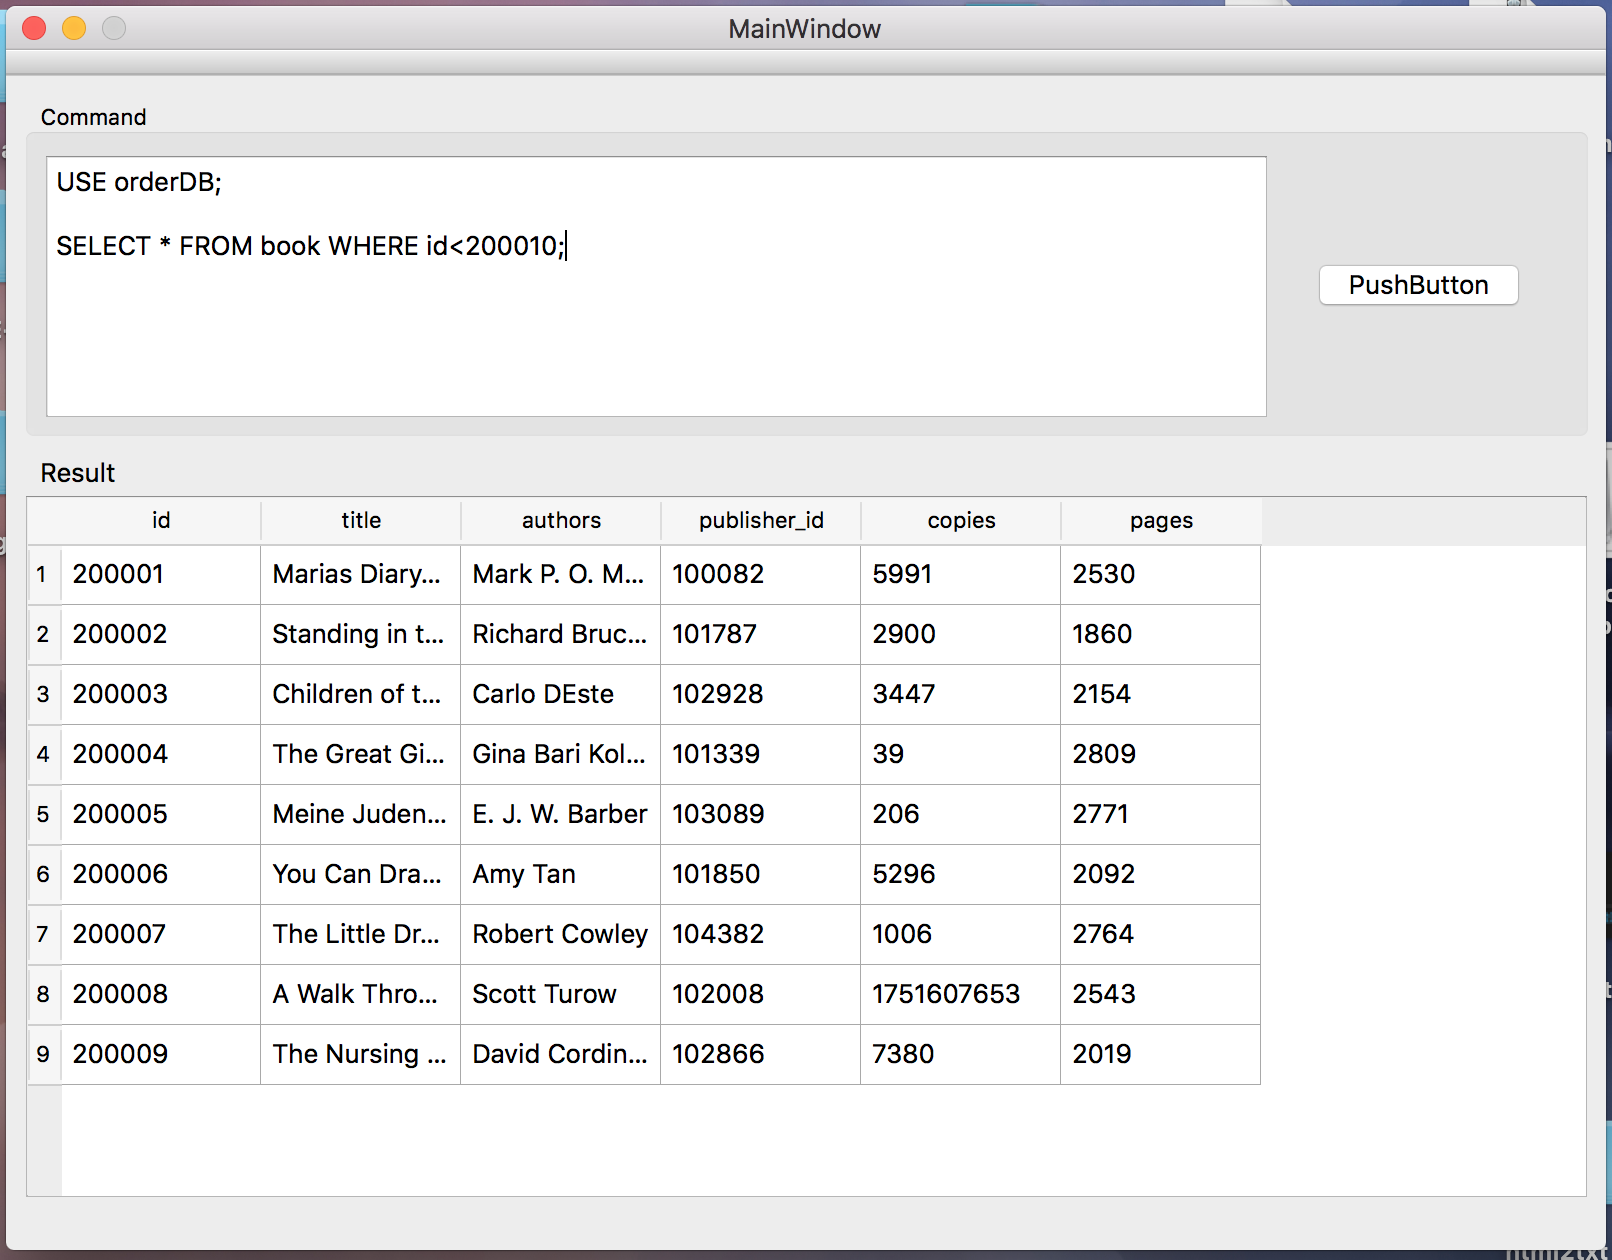
\includegraphics[width=5in]{Figures/screen_shot/basic1.png}
\end{figure}
以下是字符串类型、等于操作符:
\begin{figure}[H]
\centering
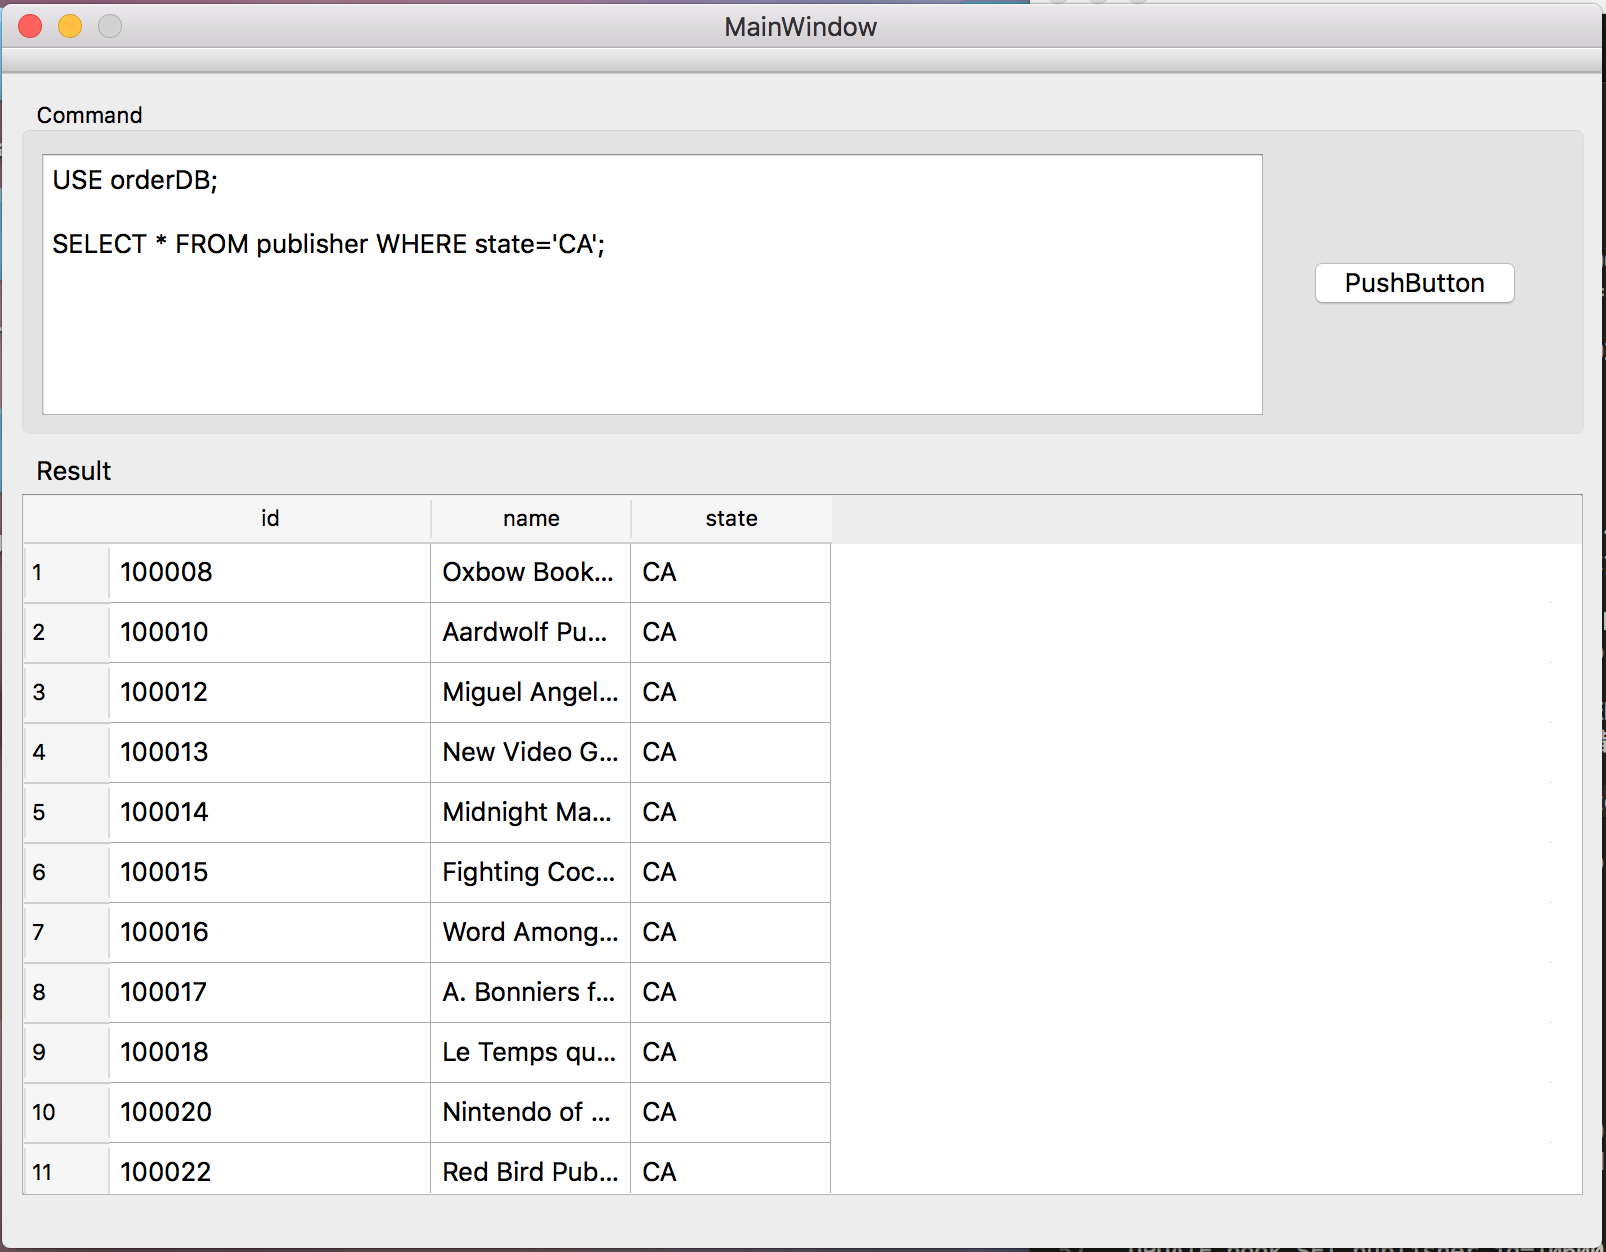
\includegraphics[width=5in]{Figures/screen_shot/basic2.png}
\end{figure}
支持复合查询条件
\begin{figure}[H]
\centering
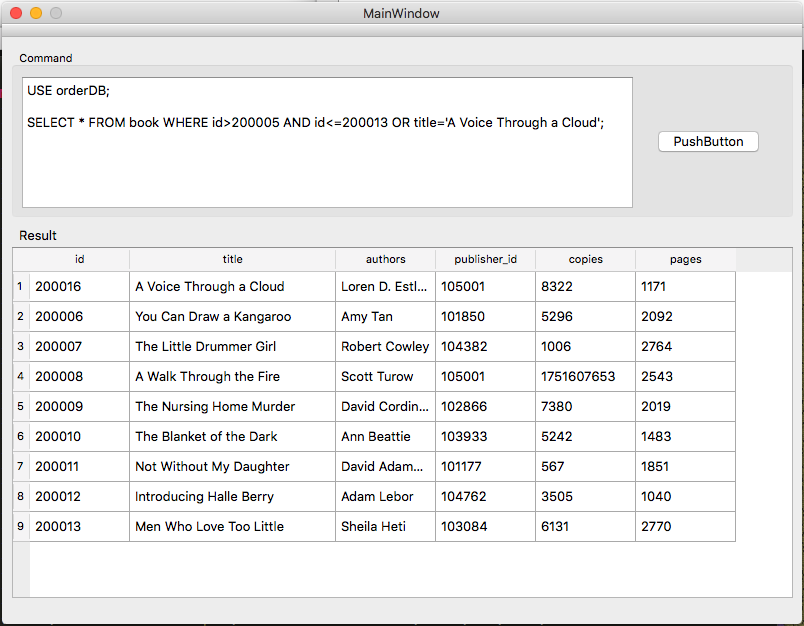
\includegraphics[width=5in]{Figures/screen_shot/where.png}
\end{figure}
支持 IS NULL的查询
\begin{figure}[H]
\centering
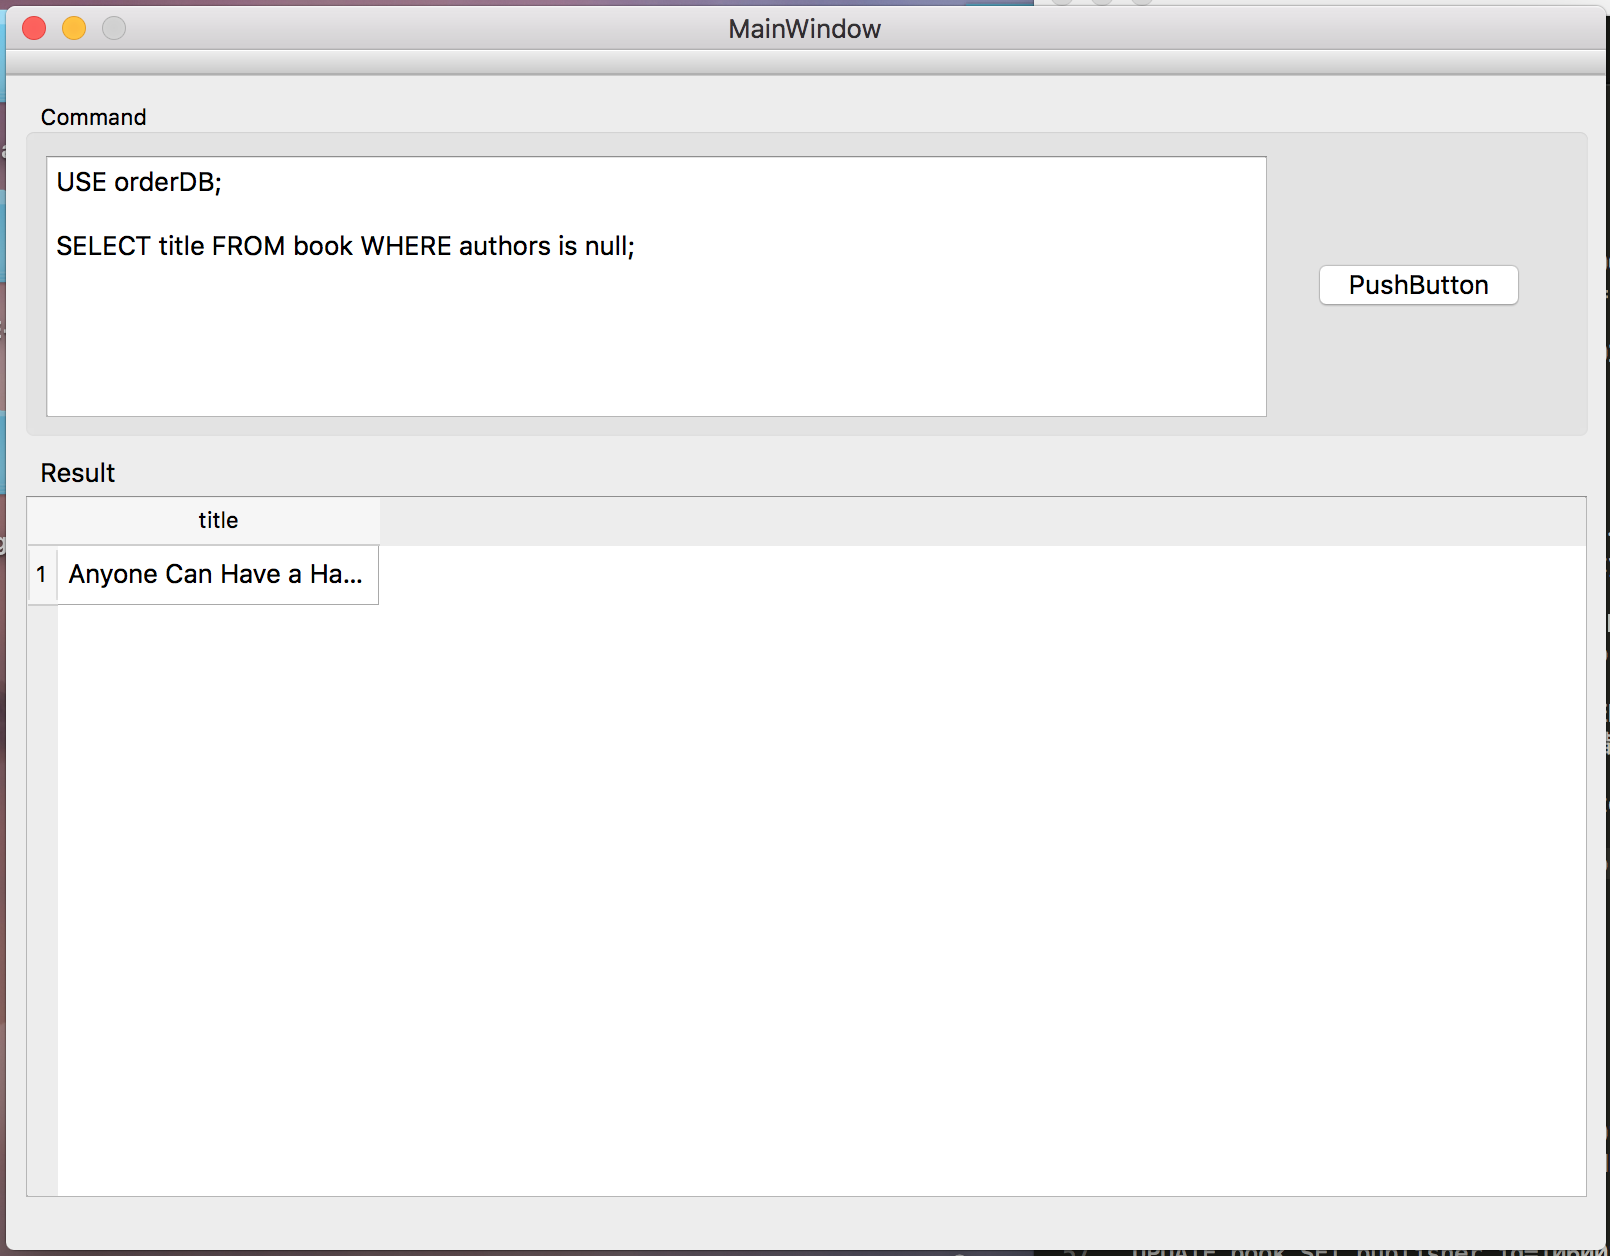
\includegraphics[width=5in]{Figures/screen_shot/isnull.png}
\end{figure}

\subsection{插入}
\begin{figure}[H]
\centering
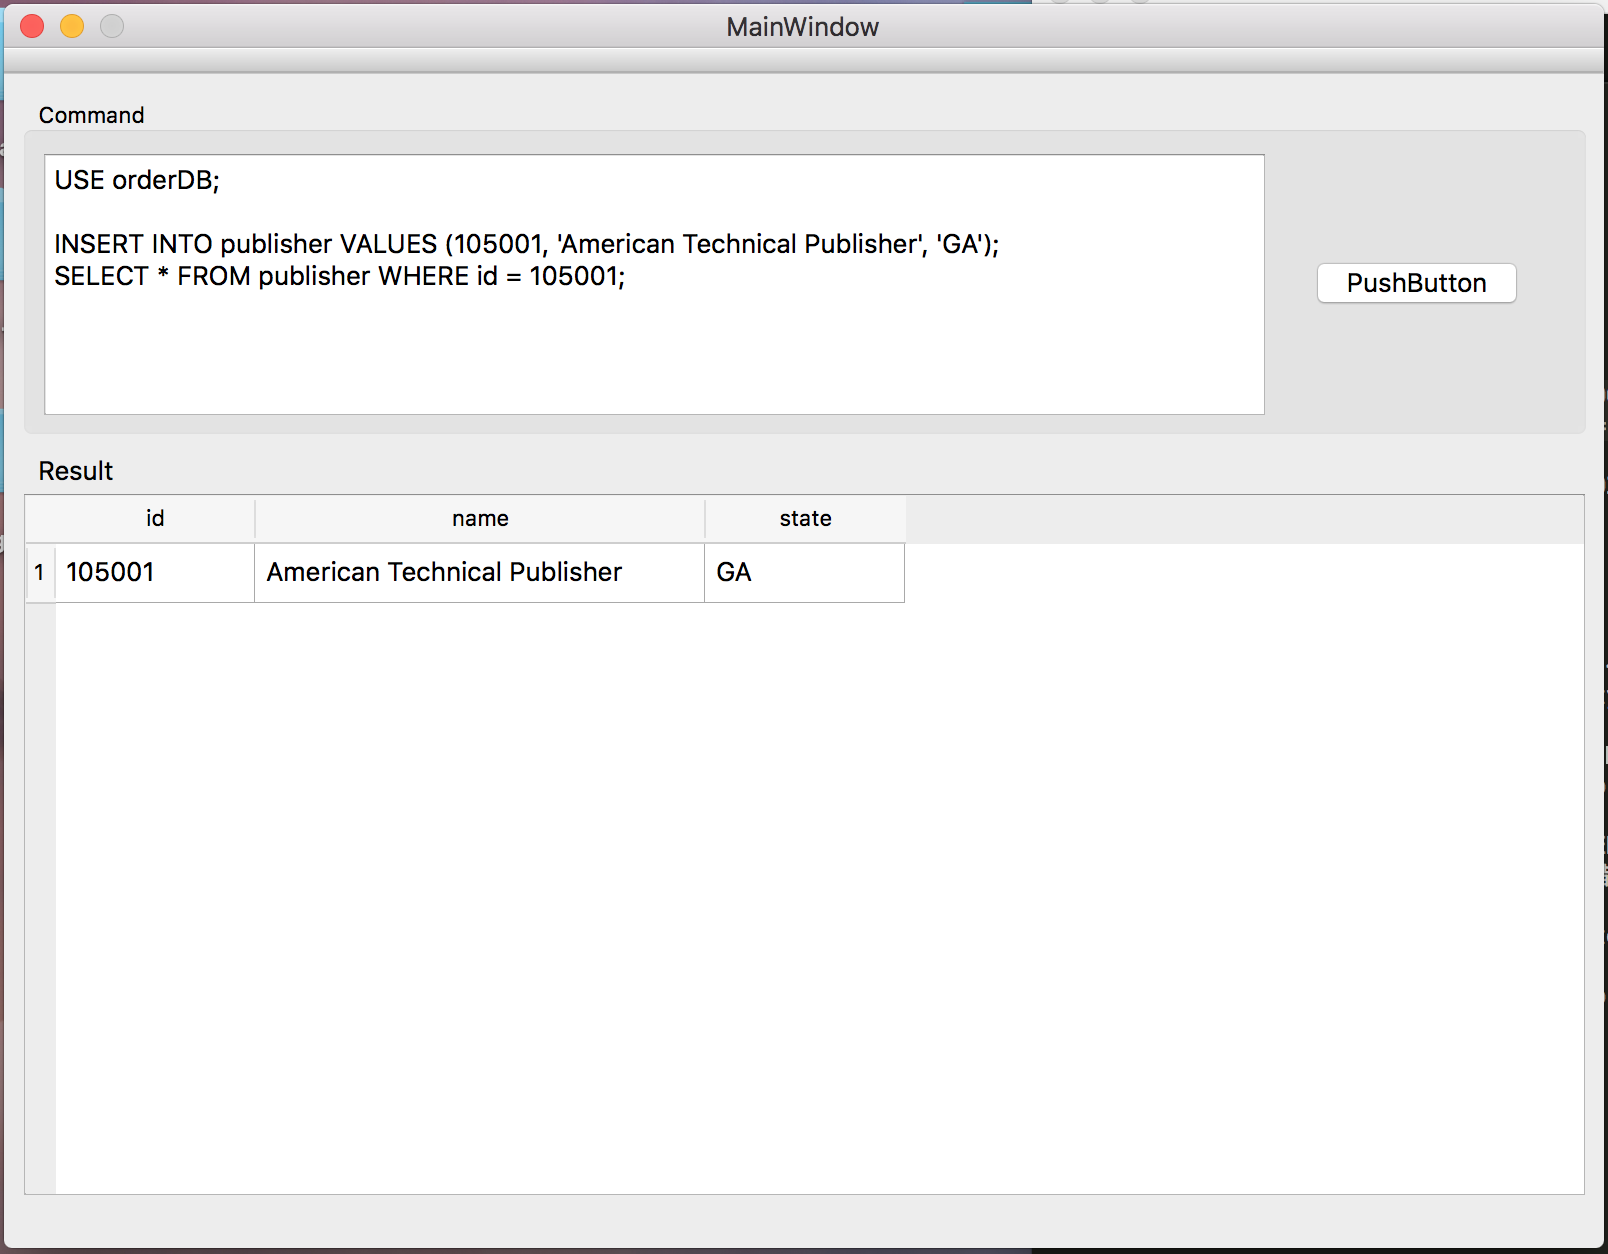
\includegraphics[width=5in]{Figures/screen_shot/insert.png}
\end{figure}

\subsection{删除}
\begin{figure}[H]
\centering
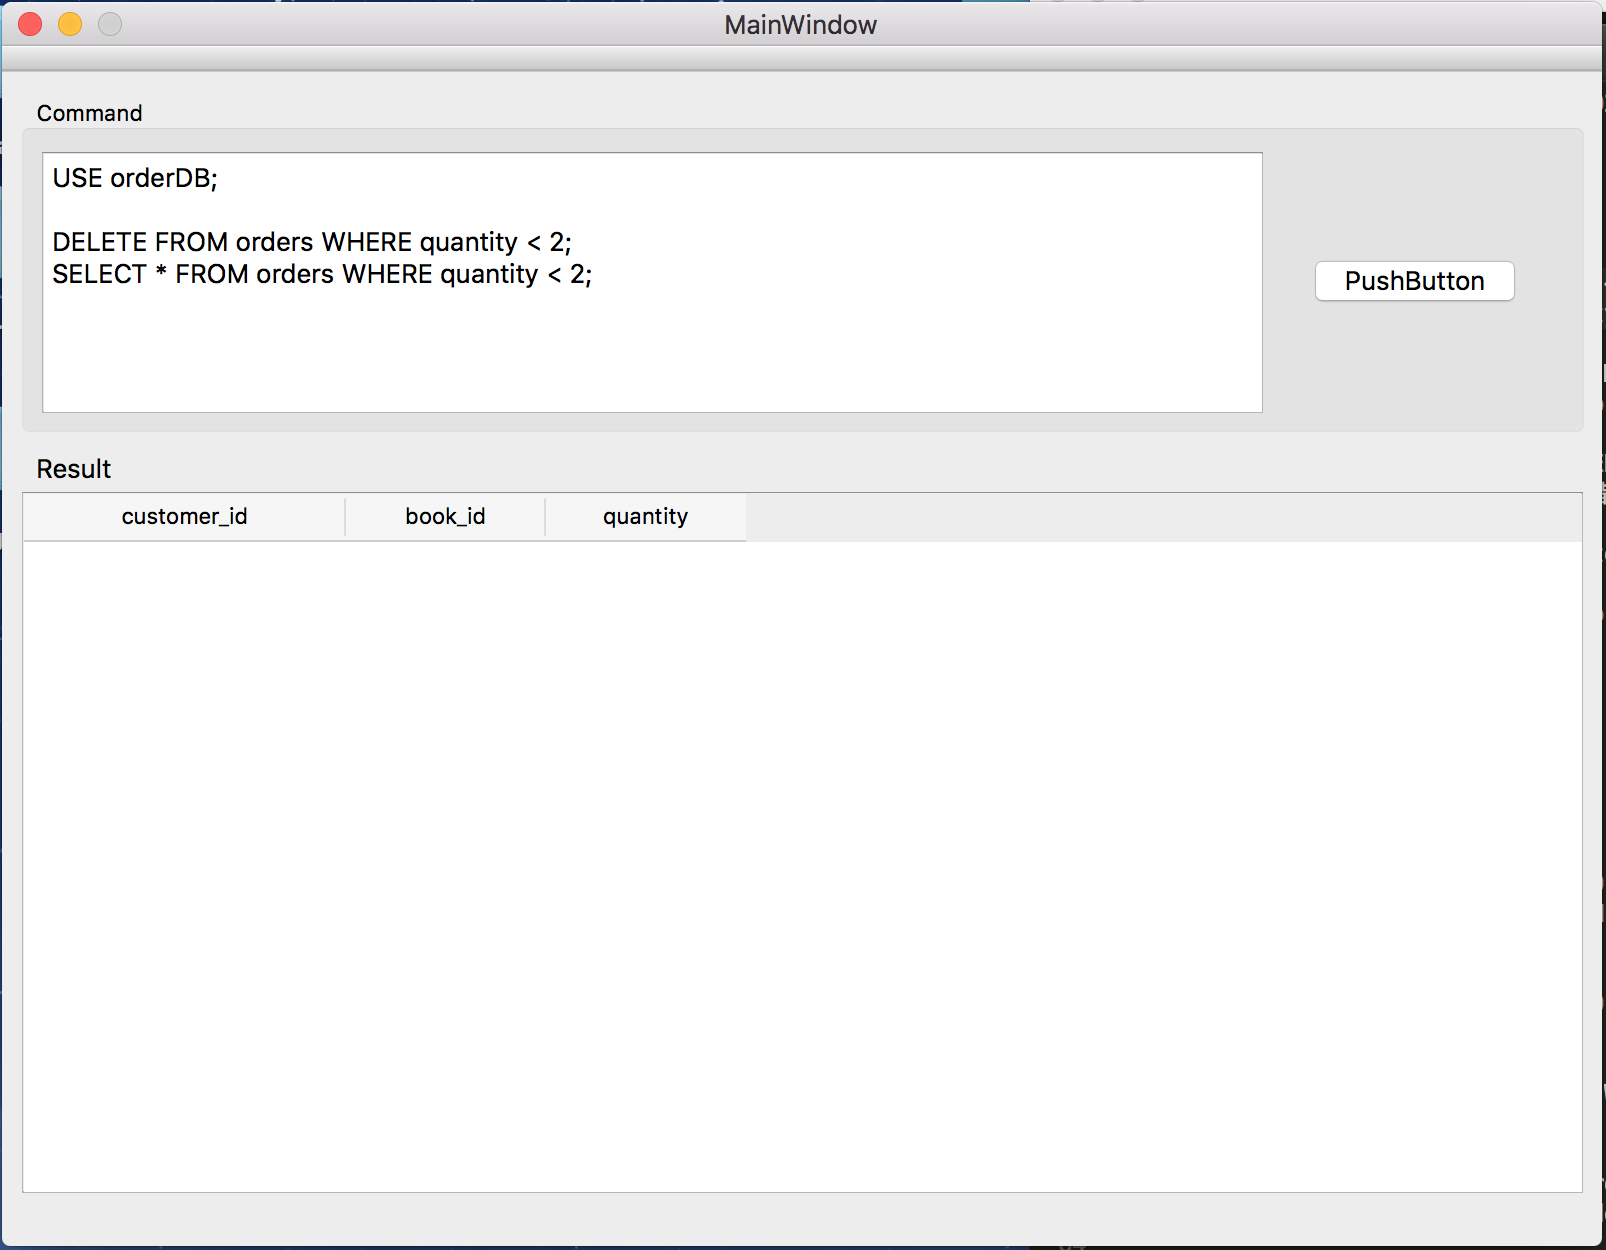
\includegraphics[width=5in]{Figures/screen_shot/delete.png}
\end{figure}

\subsection{更新}
\begin{figure}[H]
\centering
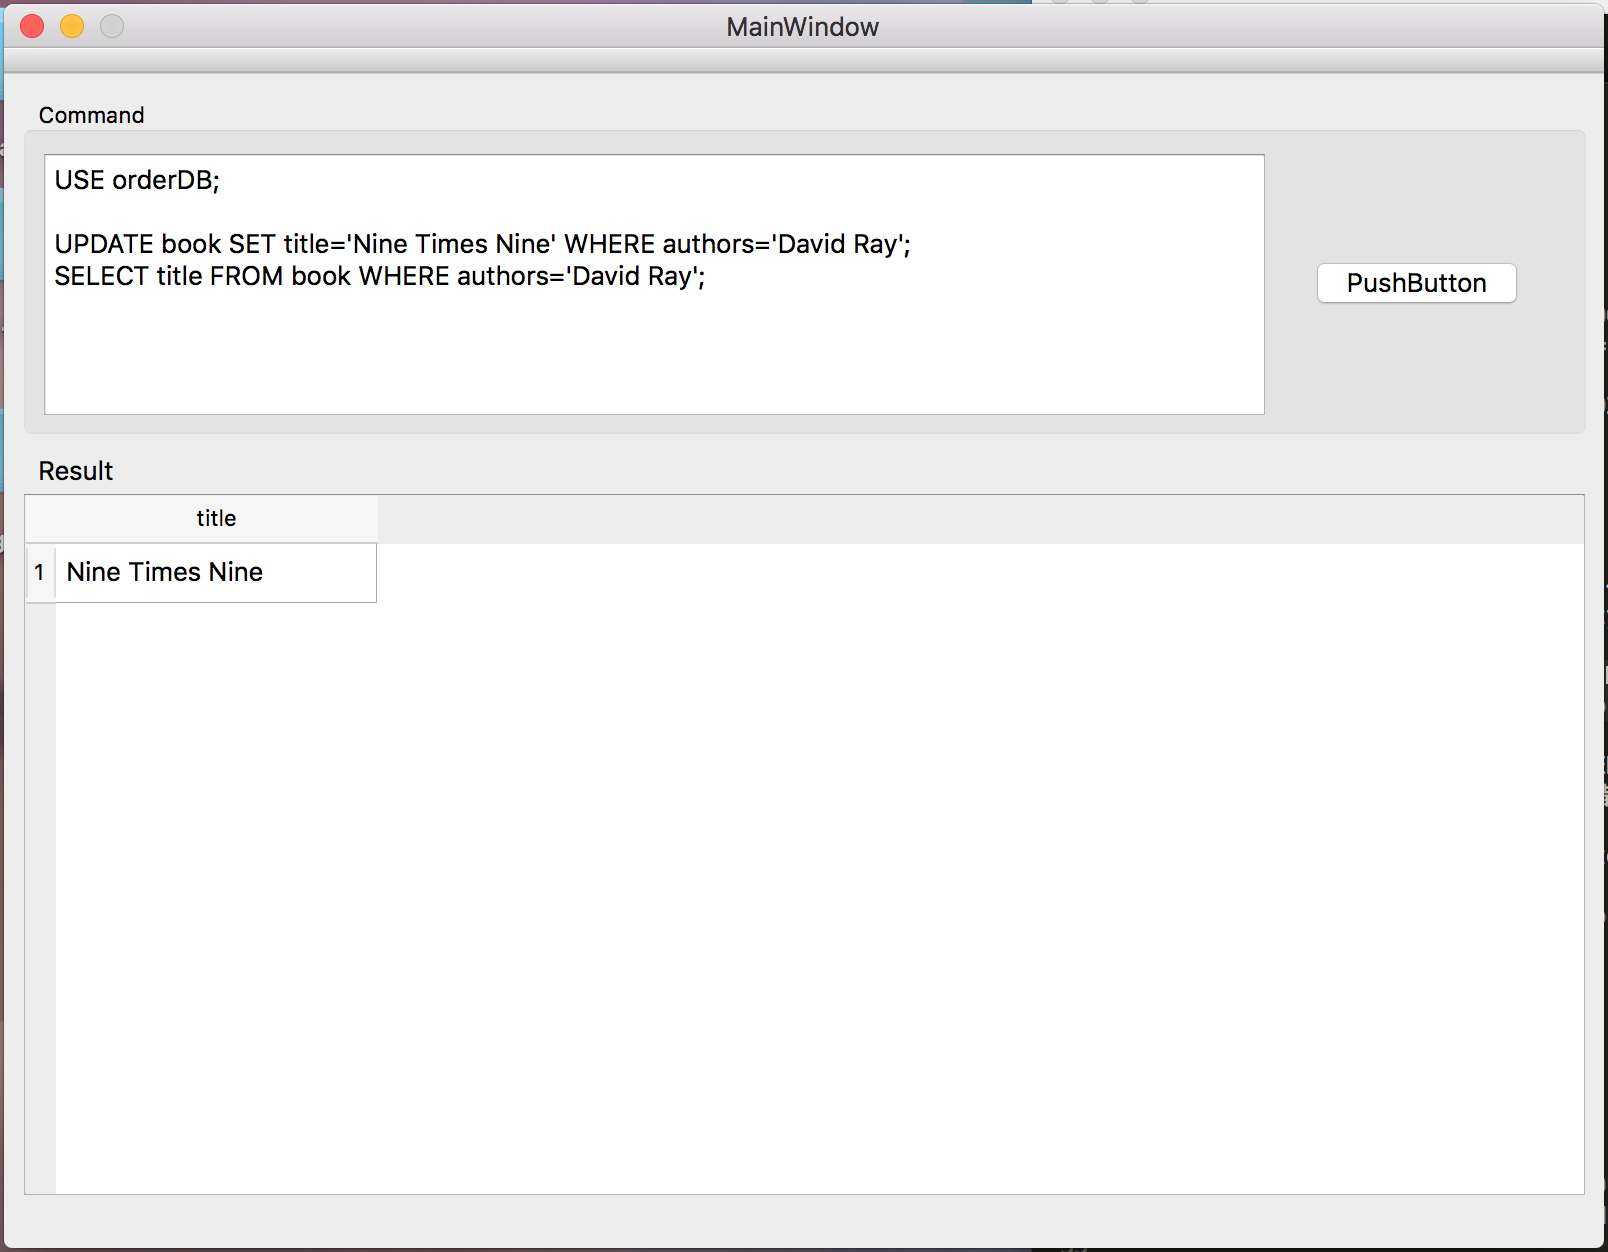
\includegraphics[width=5in]{Figures/screen_shot/update.png}
\end{figure}

\section{扩展功能}
\subsection{域完整性约束}
\begin{figure}[H]
\centering
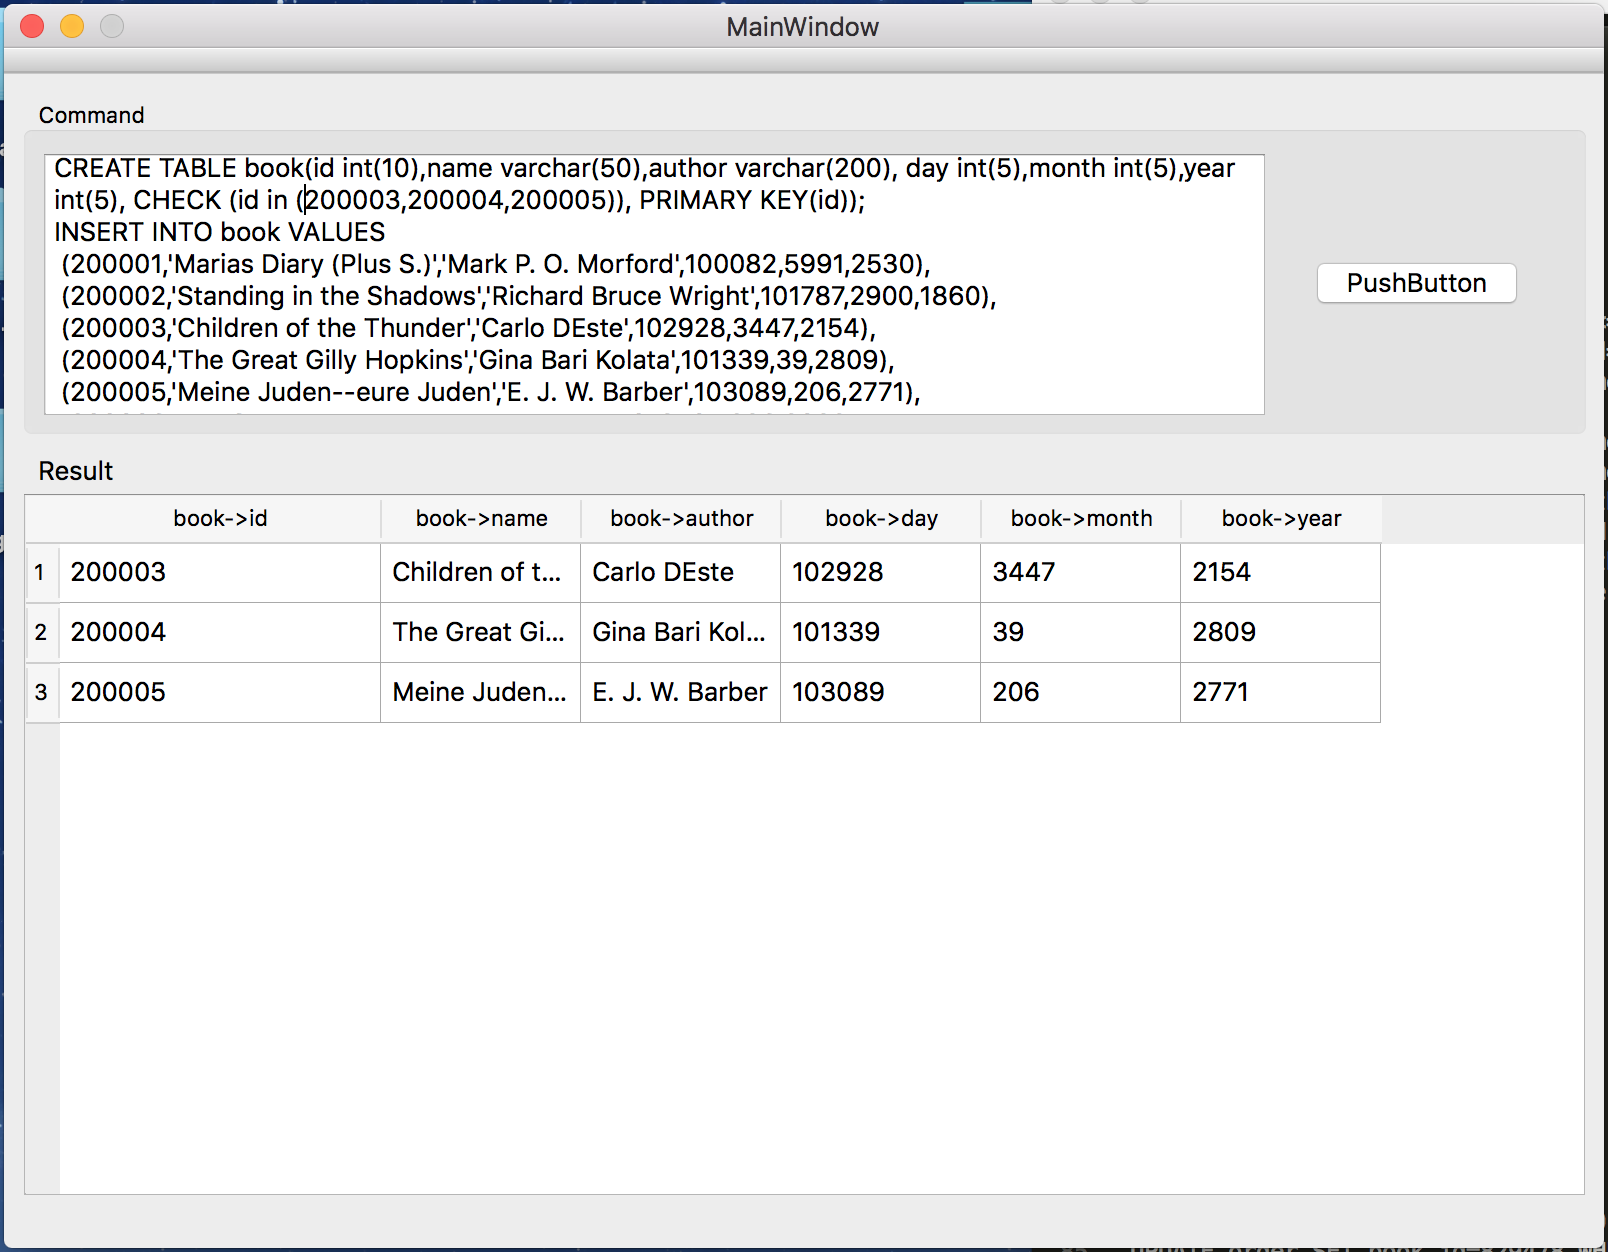
\includegraphics[width=4.75in]{Figures/screen_shot/check.png}
\end{figure}

\subsection{外键约束}
\begin{figure}[H]
\centering
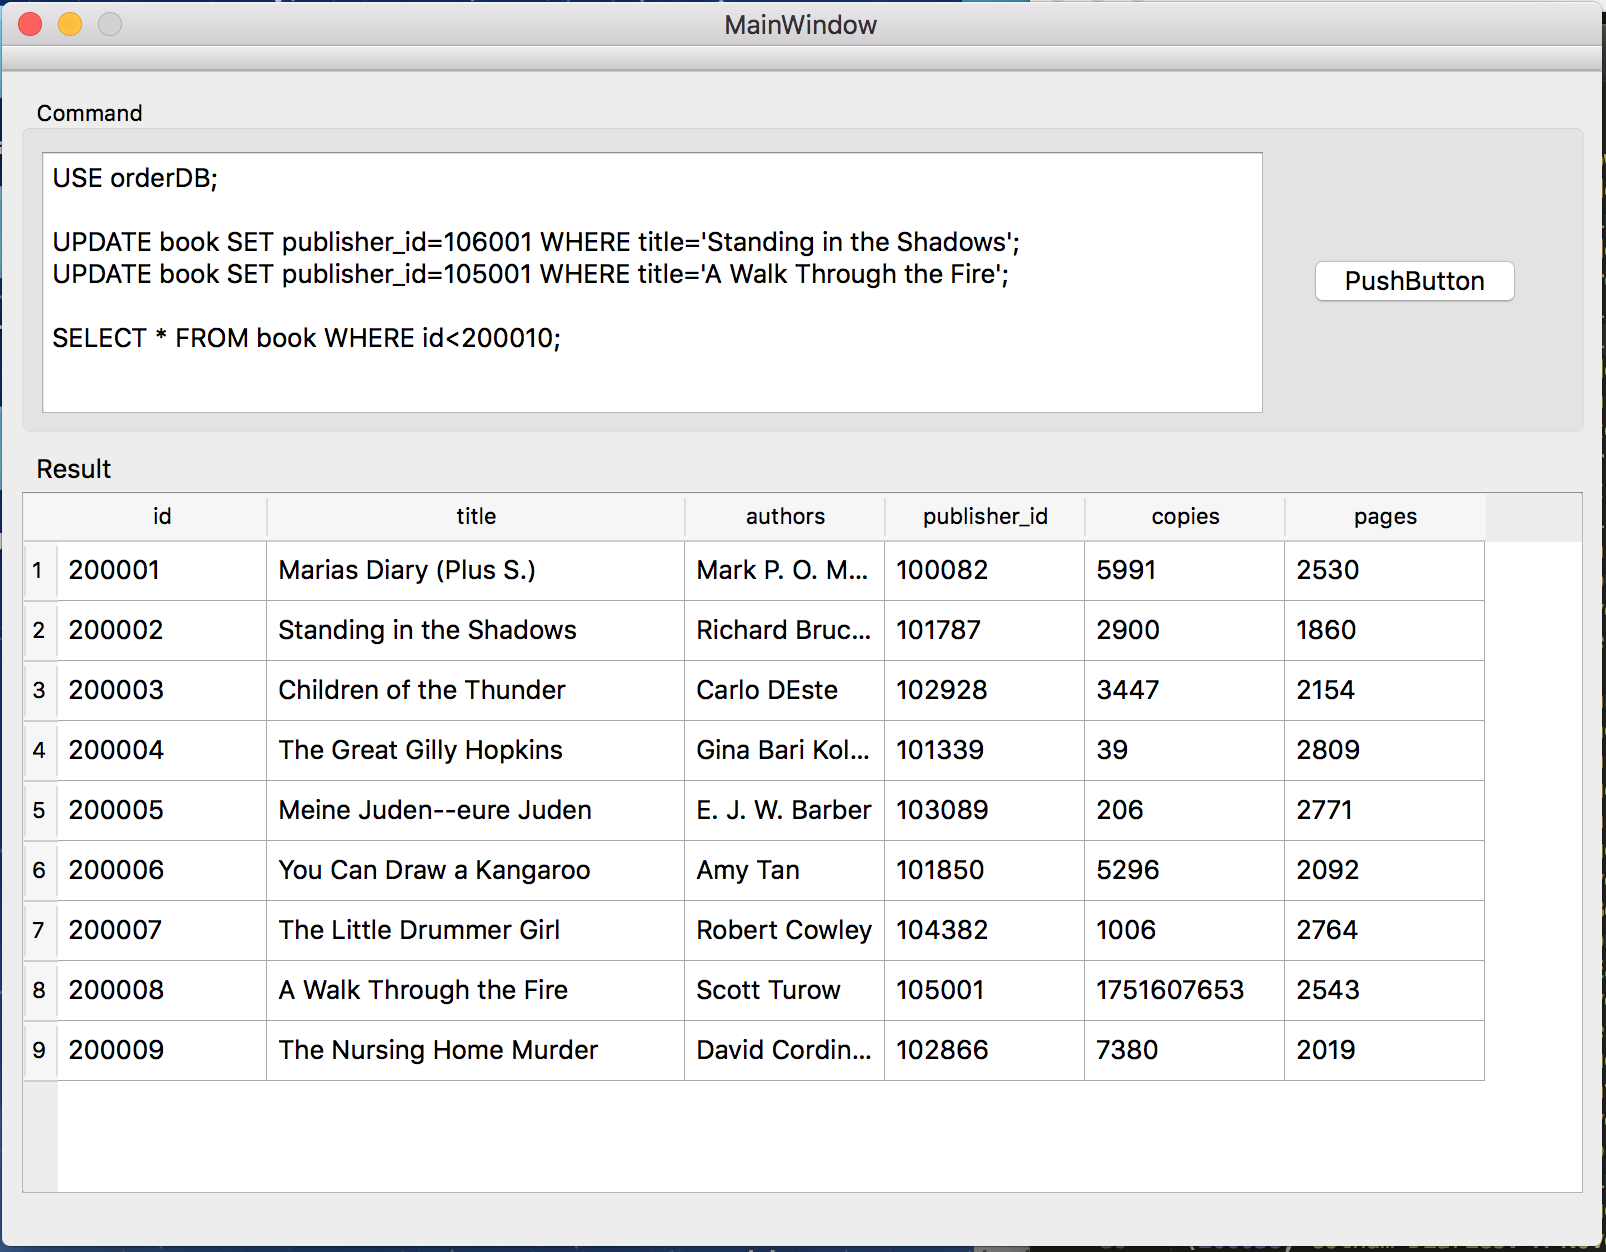
\includegraphics[width=4.75in]{Figures/screen_shot/outkey.png}
\end{figure}

\subsection{多表连接}
\begin{figure}[H]
\centering
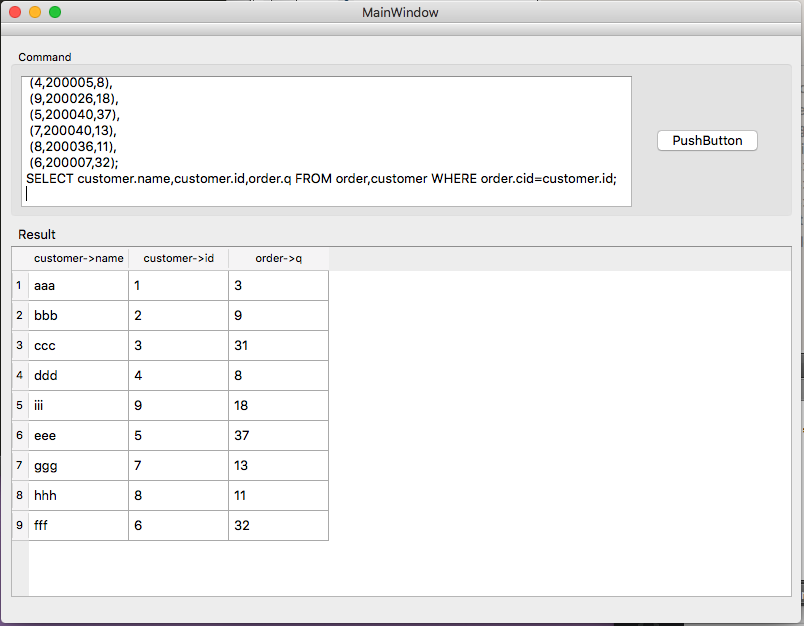
\includegraphics[width=4.75in]{Figures/screen_shot/join.png}
\end{figure}

\subsection{模糊匹配}
\begin{figure}[H]
\centering
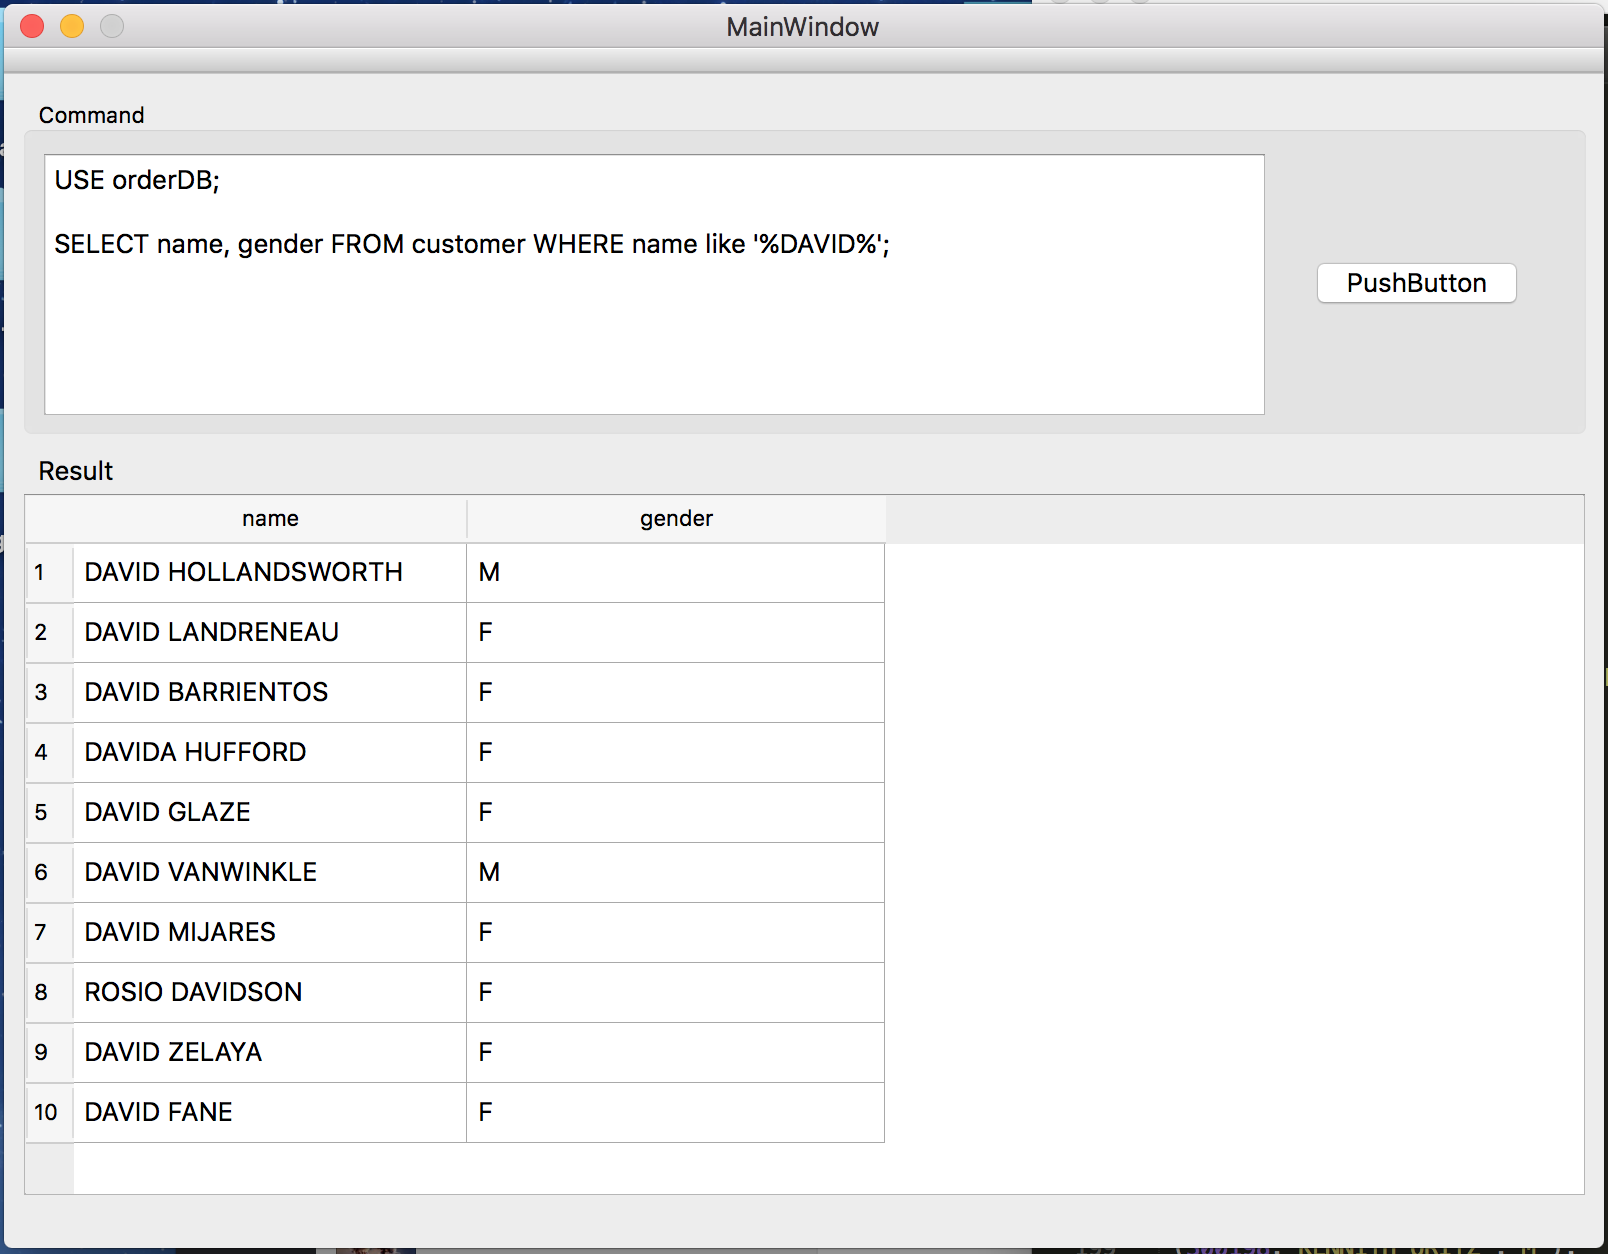
\includegraphics[width=4.75in]{Figures/screen_shot/vague.png}
\end{figure}

\subsection{聚集查询}
\begin{figure}[H]
\centering
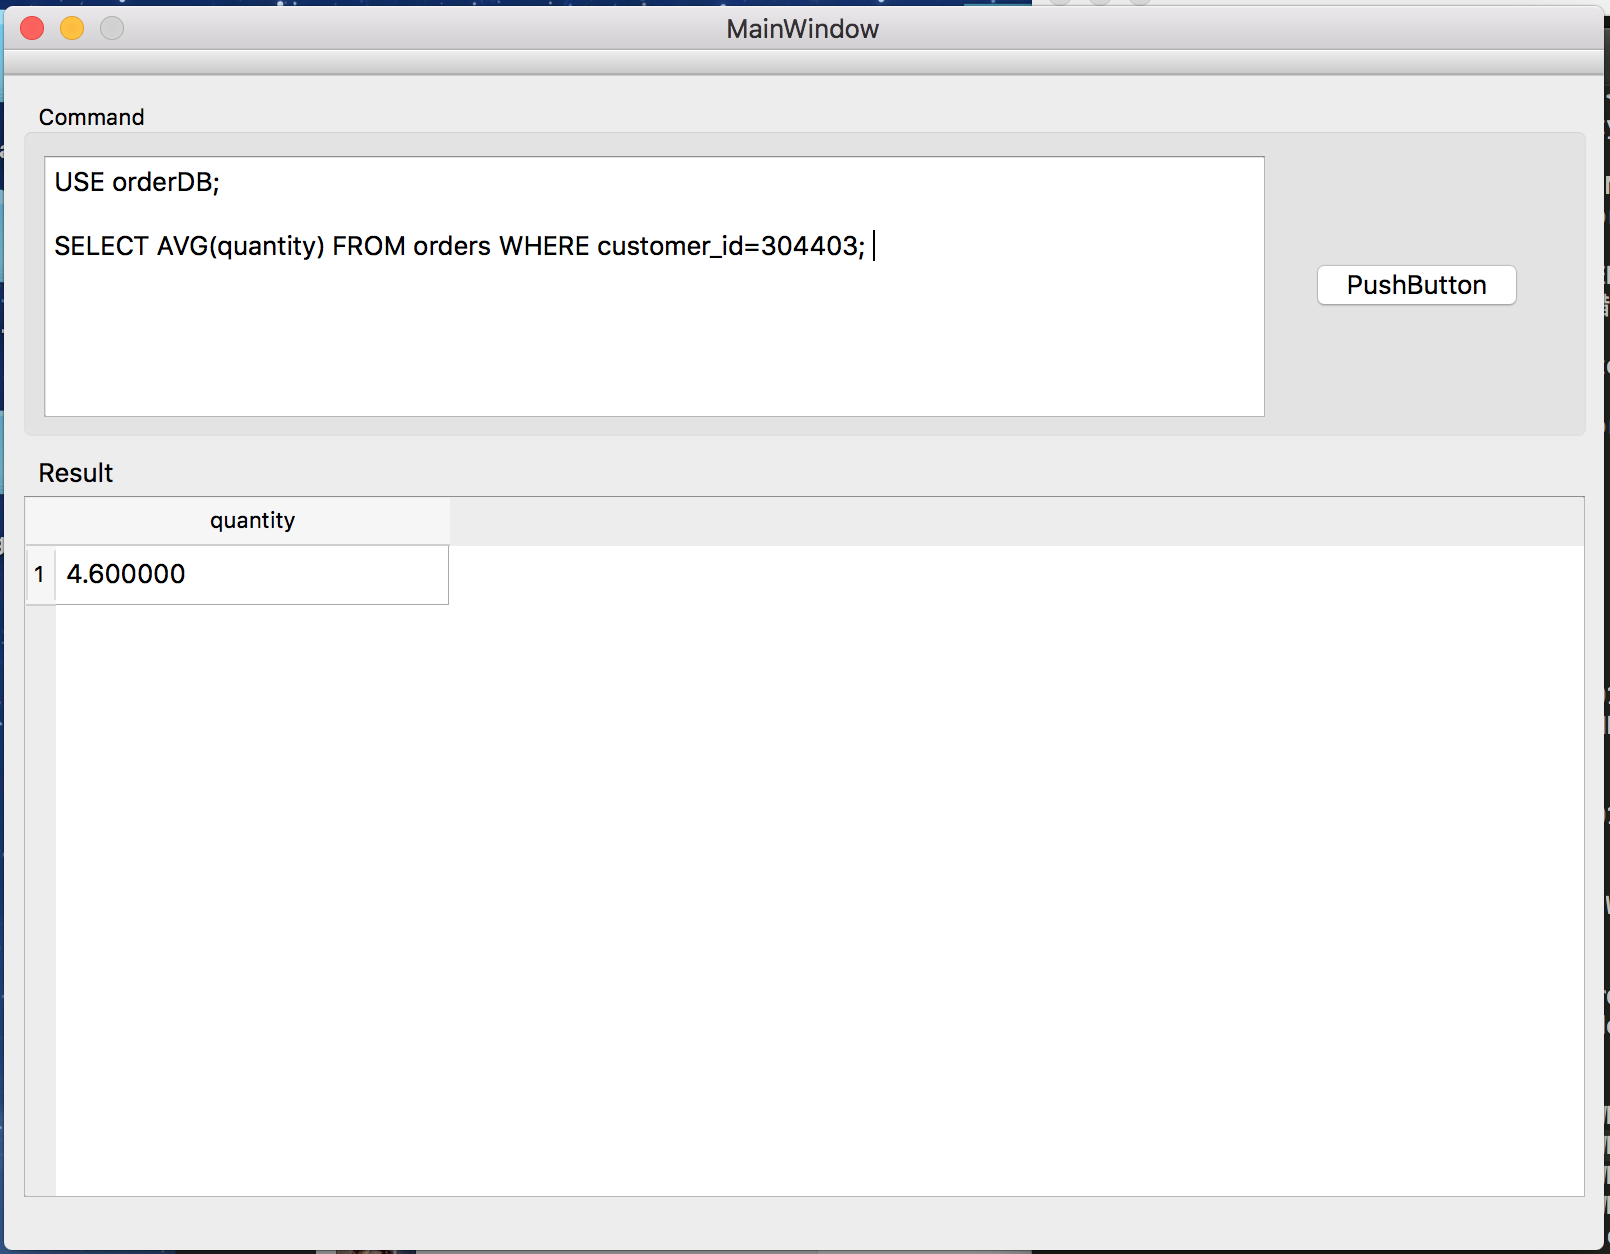
\includegraphics[width=4.75in]{Figures/screen_shot/group.png}
\end{figure}

